\chapter{The simplex method}
\label{cha:introduction}


In this chapter, we describe the simplex method. The task is to solve
a linear program 
\begin{equation}
  \label{eq:28}
  \max\{c^Tx \colon x \in \setR^n, \, Ax\leq b\}
\end{equation}
where $A \in \setR^{m\times n}$, $b \in \setR^m$ and $c \in \setR^n$. We make the
following assumption.

\dproblem{Full-rank assumption}{The matrix $A \in \setR^{m\times n}$ has full
  column-rank. In other words, the columns of $A$ are linearly
  independent}  
%
We will see later that this assumption can be made without loss of
generality. 

\section{Roofs}
\label{sec:two-variable-linear}


\begin{figure}[htbp]
  \begin{center}{
%    \psset{unit=.8cm}
    \begin{pspicture}(-4,-3)(4,4)%\showgrid
        \pspolygon[fillcolor=vlg,fillstyle=solid](-1,-2)(-2,1)(-1,2)(2,1)(1,-1)
        \psline(-4,1)(0,4)
        \psline(-2,4)(4,0)
%        \psline(-4,2)(4,4)
        \psline(-4,-1)(1,4)
        \psline(-4,3)(4,0.333)
%      \psline{->}(0,-3)(0,3)
%      \psline{->}(-3,0)(3,0)
%      \rput(-.5,-.5){$(0,0)$}
     % \psdot(2,2)
     % \psdot(1,-1)
     % \psdot(-1,-2)
     % \psdot(-.5,-1.2)
     % \psdot(.5,1.5)
     % \psdot(-2,1)
     % \psdot(-1,2)
        \psline[linecolor=red]{->}(3.5,1)(3.5,3)
        \psdot[linecolor=blue](-1,2)
        \psdot[linecolor=blue](-.95,3.3)
        \psdot[linecolor=green](3,.65)
        \rput(3,2){\red{$c$}}
    \end{pspicture}
    }
    
  \end{center}
  \caption{A linear program; the objective function vector $c$ is
    pointing vertically upwards. The blue dots mark two roofs. Notice
    that the lowest roof is the optimum of the linear program. The
    green point marks a non-roof. The two constraints
    satisfy~\ref{xitem:5}) and~\ref{xitem:6}) but not~\ref{xitem:7}). }
\end{figure}


Roofs are linear programs originating from~\eqref{eq:28} by selecting
a subset of the inequalities only. A roof should provide an upper
bound on the optimal value of the linear program~\eqref{eq:28} and at
the same time consist of $n$ ``linearly independent
constraints''. Here is the definition of a roof. 



\begin{definition}
  Consider the linear program~\eqref{eq:28} and let $B\subseteq\{1,\ldots,m\}$ be
  a subset of the row-indices. This set $B$ is a \emph{roof} if 
  \begin{enumerate}[i)]
  \item $|B| = n$, \label{xitem:5}
  \item The rows $a_i, \, i \in B$ are linearly independent, and  \label{xitem:6}
  \item The linear program  \label{xitem:7}
    \begin{equation}
      \label{eq:29}
      \max\{c^Tx \colon a_i^Tx \leq b(i), \, i \in B\}
    \end{equation}
    is bounded. 
  \end{enumerate}

\end{definition}







% \begin{figure}[htbp]
%   \centering
  
%   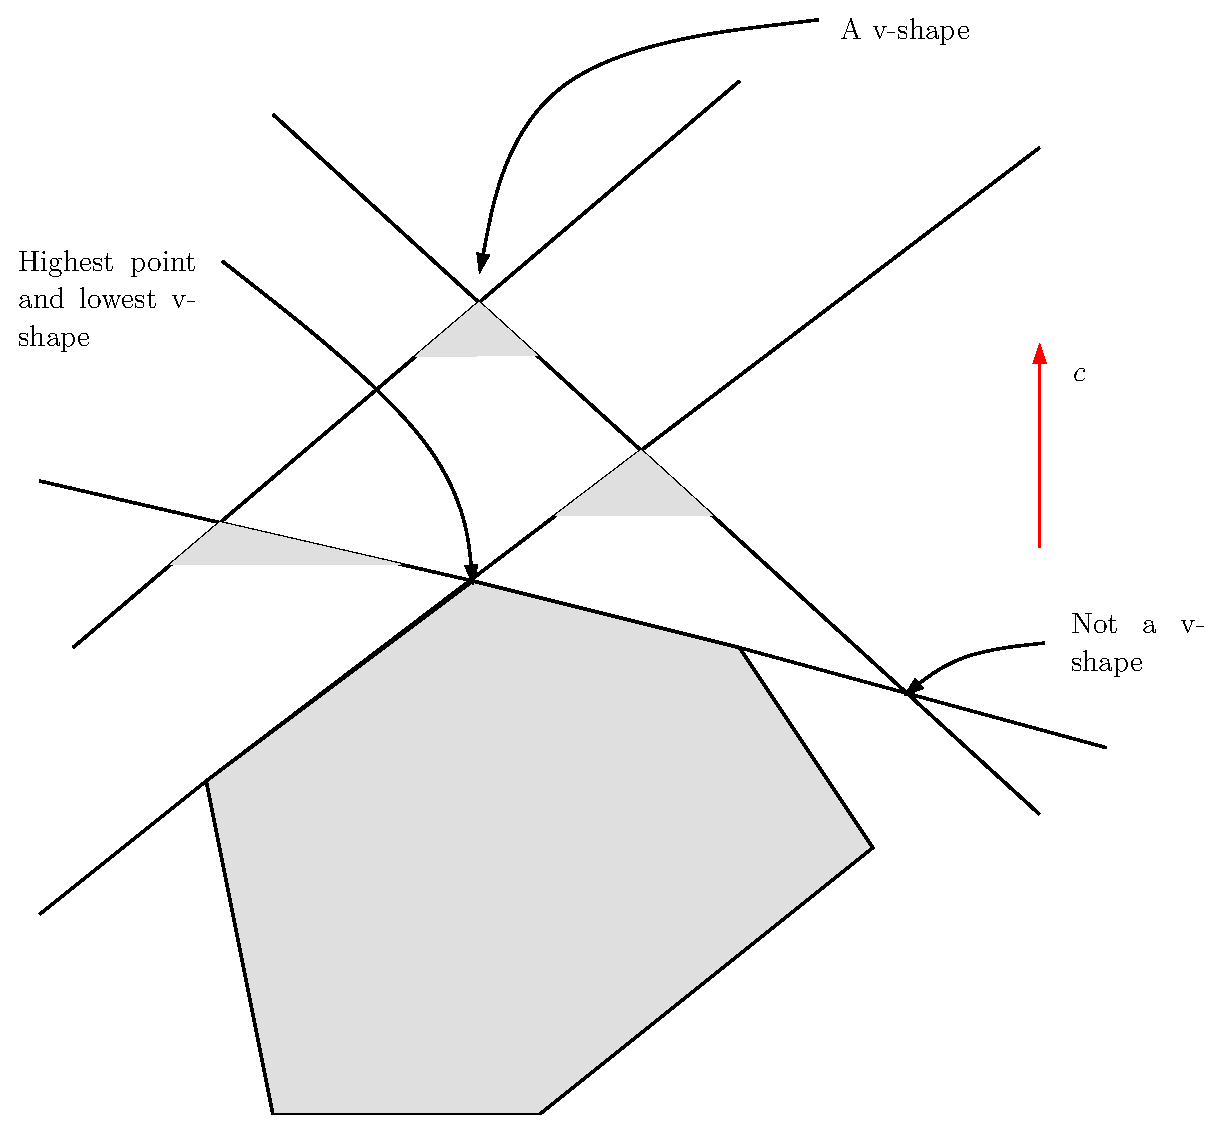
\epsfig{file=figures/highest_point.eps,height=10cm}
%   \caption{Roofs  and the optimal point}
%   \label{fig:highest_point}
% \end{figure}








\begin{figure}[htbp]
  \begin{center}{
%    \psset{unit=.8cm}
    \begin{pspicture}(-4,1)(4,4)%\showgrid
        \pspolygon[fillcolor=vlg,linecolor=vlg,fillstyle=solid](-4,1)(-1,3.25)(2,1)
        \psline(-4,1)(0,4)
        \psline(-2,4)(2,1)

         \psline[linecolor=green](-1,3.25)(-2.8,1)
        
        \psline[linecolor=red]{->}(3.5,1)(3.5,3)
%        \psdot[linecolor=blue](-1,2)
        \psdot[linecolor=blue](-1,3.25)
        \psdot[linecolor=blue](-2,2)
       % \psdot[linecolor=green](3,.65)
        \rput(-.5,3.25){$x^*_B$}
        \rput(-1.5,2){$y^*$}
       
    \end{pspicture}
    }
    
  \end{center}
  \caption{An illustration for the proof of Lemma~\ref{lem:2}. The
    green ray illustrates the set $\{x^*_B + \lambda( y^* - x^*_B) \colon \lambda \in
  \setR_{\geq0}\}$. }
\end{figure}



\noindent 
What is the optimal solution of a linear program~\eqref{eq:29} defined
by a roof? This question is answered in the next lemma. 

\begin{lemma}
  \label{lem:2}
  Let $B\subseteq\{1,\ldots,m\}$ be a roof of the linear program~\eqref{eq:28}
  and let $x^*_B$ be the unique solution of the linear system 
  \begin{displaymath}
    a_i \,x = b(i), \, i \in B,
  \end{displaymath}
  then $x^*_B$ is an optimal solution of the roof-linear
  program~\eqref{eq:29}.
\end{lemma}


\begin{proof}
  Suppose that $y^*$ is a feasible solution of the roof-linear program
  with $c^Ty^*>c^Tx^*_B$. We now show that each $x_B^* + \lambda (y^* -x_B^*)$
  for $\lambda\geq0$ is feasible. One has $a_i\, (x_B^* + \lambda (y^* -x_B^*)) =
  b(i) + \lambda\cdot ( a_i\,y^* -  b(i) ) \leq b(i)$ for each $i \in B$ and thus
  $x_B^* + \lambda (y^* -x_B^*)$ is feasible for each $\lambda\geq0$. 
  
  The objective function value of such a point  is $c^Tx_B^* +
  \lambda(c^Ty^*-c^Tx^*_B)$ which, for $\lambda \to \infty$ tends to infinity. This
  is a contradiction to $B$ being a roof
  (condition~\ref{xitem:7}). Thus $x^*_B$ must be  an optimal 
  solution to the roof-linear program~\eqref{eq:29}.   \qed
\end{proof}


Now that we know that a roof-linear program has an optimal solution,
we can define the value of a roof $B$.

\begin{definition}
  The \emph{value}  of a roof $B$ is the optimum value $c^Tx^*_B$ of
  the roof-linear program
  \begin{displaymath}
    \max\{c^Tx \colon a_i\,x\leq b(i), \, i \in B\}. 
  \end{displaymath}
\end{definition}



The next theorem is very simple, but in fact very important. It states
that the value of a roof is an upper bound on the optimum value of a
linear program $\max\{c^Tx \colon x \in \setR^n, \, Ax\leq b\}$. 

\begin{theorem}[Weak duality]
  \label{thr:6}
  The value of a roof is an upper bound on the objective function
  value of any feasible point of the linear program.   
\end{theorem}


\begin{proof}
  Let $B$ be a roof of the linear program $\max\{c^Tx \colon x \in \setR^n, \,
  Ax\leq b \}$. Any feasible point $x^*$ of this linear program is also
  a feasible point of the 
  roof-linear program $\max\{c^Tx \colon a_i\,x\leq b(i)\}$. Therefore
  $c^Tx^*_B \geq c^Tx^*$ and the claim follows. \qed 
\end{proof}


When is an index-set $B\subseteq\{1,\ldots,m\}$ satisfying  \ref{xitem:5}) and
\ref{xitem:6}) a roof? Consider the  example in see
Figure~\ref{fig:2}. The objective is 
to maximize $2x_1+x_2$ and the two roof-constraints are $x_1+x_2\leq5$
and $x_1\leq6$. From the picture, it is clear that the objective
function vector is in the cone of the two constraint vectors. In fact,
this is the characterization that holds in any dimension as we now
show. 






\begin{figure}[htbp]
  \begin{center}{
%    \psset{unit=.8cm}
    \begin{pspicture}(-1,-2)(5,4)
      \pspolygon[fillcolor=vlg,linecolor=vlg,fillstyle=solid](-1,4)(2,1)(2,-2)
      \psline(2,-2)(2,4)
      \psline(-1,4)(4,-1)
      \psline[linecolor=red]{->}(2.5,1.5)(4.5,2.5)
      \psline[linecolor=blue]{->}(0,3)(1,4)
      \psline[linecolor=blue]{->}(2,-1)(3,-1)
%      \showgrid
    \end{pspicture}

    \vspace{1cm}
    \begin{pspicture}(0,0)(4,4)
%      \rput(-.2,-.2){$0$}
      \pspolygon[fillcolor=vlg,linecolor=vlg,fillstyle=solid](0,0)(4,0)(4,4)
       \psline[linecolor=red]{->}(0,0)(2,1)
      \psline[linecolor=blue]{->}(0,0)(1,0)
      \psline[linecolor=blue]{->}(0,0)(1,1)
%      \showgrid
    \end{pspicture}
    }
    
  \end{center}

  \caption{A roof that is defined by the two constraints $x_1\leq2$ and
    $x_1+x_2\leq3$. The objective function  vector is $(2,1)^T$. Indeed
    $(1,1)^T = 1 \cdot (1,1)+ 1\cdot (1,0)$ which shows that it is in the
    cone generated by the constraint-defining vectors.  
    }
  \label{fig:2}
\end{figure}






\begin{lemma}
  \label{lem:4}  
  Let $B\subseteq\{1,\ldots,m\}$ satisfy \ref{xitem:5}) and
  \ref{xitem:6}). Then $B$ is a roof, if and only if $c \in \cone\{a_i\colon i \in B\}$. 
\end{lemma}

\begin{proof}
  Suppose that $c \in \cone\{a_i\colon i \in B\}$. Thus there exist
  $\lambda_i\geq0, \, i\in B$ with $c = \sum_{i \in B}\lambda_i\cdot a_i$. 
  The  unique solution $x^*_B$  to the
  system 
  \begin{equation}
    \label{eq:0}
    a_i\,x=b(i), \, i\in B
  \end{equation}
  is an optimal solution to
  $\max\{c^Tx \colon a_i\,x\leq b(i)\}$. Because if $\wt{x}$ is another feasible solution,
  then $c^T\wt{x} = \sum_{i\in B} \lambda_i \cdot a_i\, \wt{x}$. Since $\lambda \geq0$ and
  $a_i\,\wt{x}\leq b(i)$  we can write
  \begin{eqnarray}
    \label{eq:2}
    c^T\wt{x} & = &  \sum_{i\in B} \lambda_i\cdot a_i\,  \wt{x}\\
    & \leq & \sum_{i\in B} \lambda_i\cdot  b(i) \\
    & = &  \sum_{i\in B} \lambda_i\cdot  a_i\,x_B^*\\
    & = &  (\sum_{i\in B} \lambda_i\cdot  a_i )\, x_B^*\\
             & = & c^Tx_B^*.
  \end{eqnarray}
  Thus $B$ is a roof. 

  Suppose on the other hand that $B$ is a roof.  Then, since
  $a_i, i\in B$ is a basis of $\setR^n$, there exist $y_i \in  \setR, \, i \in B$ with 
  $c =  \sum_{i \in B}y_i \cdot a_i$. If all $y_i\geq0, \, i \in B$, then it
  follows that $c \in \cone\{a_i \colon i \in B\}$ and we are done. 
  Suppose therefore   that there exists an index  $j \in B$ with
  $y_{j}<0$. We will derive a contradiction. 

% Without loss of 
  %  generality assume  $y(1)<0$. 
  Consider the system of linear equations
  \begin{equation}
    \label{eq:1}
    a_{j}\,x = -1, a_i\,x=0, \, i \in B\setminus\{j\}. 
  \end{equation}
  This system~\eqref{eq:1} has a unique solution $0\neq v\in \setR^n$.  
  Let $x^*$ be a feasible solution to the roof-linear
  program. Clearly $x^* + \lambda \cdot v$ is also feasible for each 
  $\lambda>0$ (Exercise~\ref{xitem:9}). But $c^T (x^* + \lambda v) = c^Tx^* + \lambda \cdot \sum_{i=1}^n y_i  a_i\,  v = c^T x^*
  + \lambda \cdot y_{j} \cdot  a_{j}\,v = c^T x^*  - \lambda \cdot y_{j} $. This increases with $\lambda$ since $y_{j}<0$ and
  $a_{j}\,v<0$.  This contradicts the fact $B$ is a roof, since the
  roof-linear program is unbounded. \qed 
\end{proof}





\begin{definition}
  \label{def:5}
  Let $B$  be a roof of the linear program~\eqref{eq:28}. The unique
  solution 
  $x^*$  of  the
  system 
  \begin{equation}
    \label{eq:3}
 a_i^Tx = b(i), \, i \in B, 
  \end{equation}
  is the  \emph{vertex} of the roof. 
\end{definition}


% The proof of Lemma~\ref{lem:4} reveals the following fact. 

% \begin{proposition}
% \label{prop:1}
% Let $\ev$ be a v-shape of $\hpp(\eh,c)$. The vertex of $\ev$ is an
% optimal solution to $\hpp(\ev,c)$.
% \end{proposition}


Similarly one can prove the following fact. 

\begin{proposition}
  \label{prop:2}
  Let $B$ be a roof of the linear program~\eqref{eq:28}. 
    The vertex of a roof is the \emph{unique optimal solution} of the
    roof-linear program~\eqref{eq:29} if and only if   
    $c$ is a \emph{strictly positive} conic combination  of 
    the normal-vectors $a_i, i \in B$. 
\end{proposition}





\section{The simplex algorithm}
\label{sec:simplex-algorithm}


We now sketch one iteration of the simplex algorithm. Our task is to
solve a linear program~\eqref{eq:28} and we assume that we have a roof
$B$ to start with.


\begin{enumerate}[i)]
\item Compute the vertex $x^*_B$ of the roof $B$. \label{xitem:13}
\item Find an index $i \in  \{1,\ldots,m\}\setminus B$ with $a_i\,x^*_B>b(i)$. If
  there does not exist such an index, then $x^*_B$ is an optimal
  solution of the linear program~\eqref{eq:28}. \label{xitem:14} 
\item Determine an index $j \in B$ such that \label{xitem:17}
  \begin{enumerate}[a)]
  \item   $B' = B \cup \{i\} \setminus \{j\}$ is a roof, and \label{xitem:15}
  \item The vertex $x^*_{B'}$ of $B'$ is feasible for $B$. \label{xitem:16}
  \end{enumerate}
  If such an index does not exist, then the linear
  program~\eqref{eq:28} is infeasible. 
\end{enumerate}


The simplex algorithm iterates these steps until it has found an
optimal solution, or asserts that the linear program~\eqref{eq:28} is
infeasible. The big questions are how to determine an index $j$ such
that \ref{xitem:15}) and \ref{xitem:16}) hold in step \ref{xitem:17}) and
that the algorithm is correct. Furthermore, we want to understand
whether the simplex method eventually terminates.  







\subsection{Termination and degeneracy}




\begin{definition}[Degenerate roof and linear program]
  \label{def:4}
  A roof $B$ of a linear program~\eqref{eq:28} is \emph{degenerate} if
  the optimum solution of the roof-linear program~\eqref{eq:29} is not
  unique. A linear program is called degenerate, if it has degenerate
  roofs. 
\end{definition}


\begin{figure}[htbp]
  \centering
  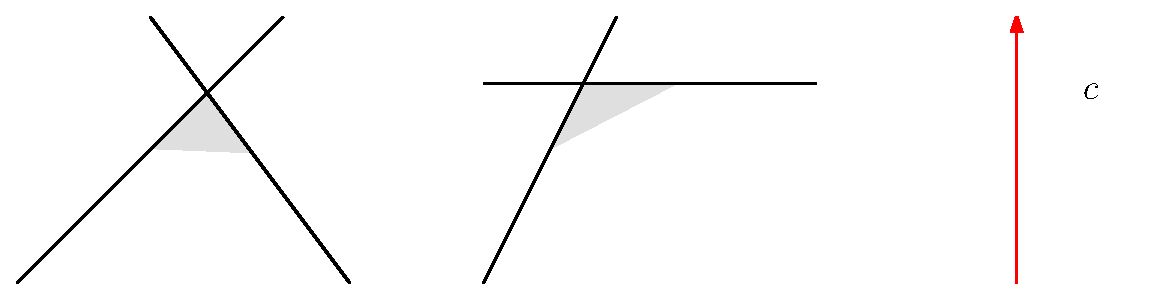
\includegraphics[height=3cm]{figures/degnodeg.eps}
  \caption{A non-degenerate and a degenerate roof.}
  \label{fig:non-deg-deg}
\end{figure}



We now argue that the simplex algorithm  terminates if the linear
program is non-degenerate. 

\begin{theorem}
  \label{thr:1}
  If the linear program~\eqref{eq:28} is non-degenerate, then the
  simplex algorithm terminates. 
\end{theorem}



\begin{proof}
  The important observation is that the simplex method makes progress
  from iteration to iteration because of the non-degeneracy of the
  roofs. If $B'$ is the roof computed in step~\ref{xitem:17}), then,
  since $x^*_{B'}$ is contained in the feasible region of the roof
  $B$, and since $B$ is non-degenerate, we have
  $c^Tx^*_B>c^Tx^*_{B'}$. Since there is only a finite number of
  roofs, the algorithm thus terminates. \qed
\end{proof}


\subsection{Implementing step~\ref{xitem:17})}


% \begin{figure}[htbp]
%   \centering
%   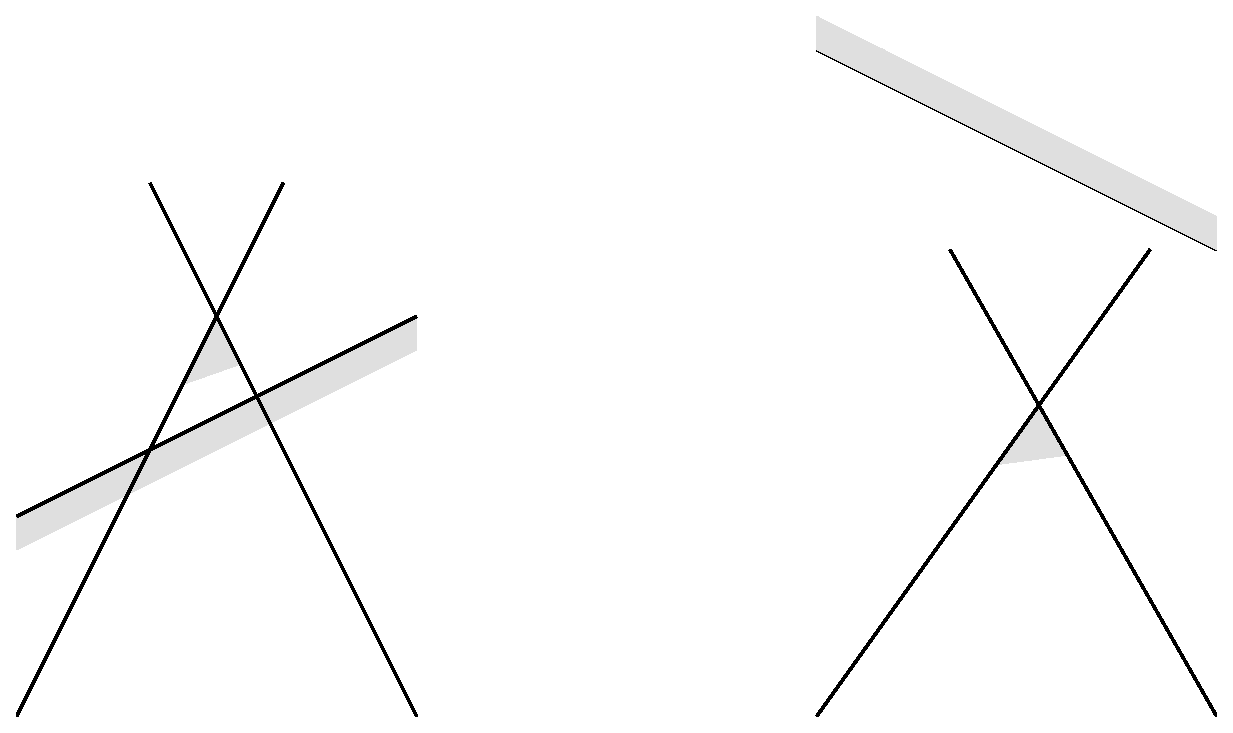
\epsfig{file=figures/entering.eps,height=5cm}
%   \caption{On the left: A strictly lower roof. On the right: $\eh$
%     is infeasible}
%   \label{fig:two-poss}
% \end{figure}


% We now describe the procedure for this move. Suppose that $a_1,\ldots,a_n$
% are the normal-vectors of the initial v-shape $\ev$.

% \noindent 
% {\bf Step 1:}  Compute the vertex $x^*$ of $\ev$. 

% \begin{lemma}
%   \label{lem:5}
%   If there exists no halfspace $h \in \eh$ which is violated by $x^*$,
%   then $x^*$ is an optimal solution to the highest point problem. 
% \end{lemma}

% \begin{proof}
%   Easy!
% \end{proof}

% \noindent
% {\bf Step 2:} Find a halfspace $a\,x\leq\beta$ for which $x^*$ is not
% feasible. If such a halfspace does not exist, then $\ev$ is a lowest
% v-shape and we stop.   

The situation is as follows. We are having a roof $B$ and its vertex
$x^*_B$ and an index $i \in \{1,\ldots,m\}$ with $a_i\,x^*_B> b(i)$. We now
want to bring $i$ into the new roof and we have to determine a $j \in
B$ that is supposed to leave the roof. The idea is very similar now to
the proof of Carath\'eodory's theorem. 

Consider the systems of equations 
\begin{eqnarray}
  \sum_{k \in B} a_k z_k   & = &  c^T \label{eq:5}\\
  \sum_{k \in B}  a_k y_k   & = &  -a_i \label{eq:17}
\end{eqnarray}
with variables $z_k, \, k \in B$ and $y_k,\, k \in B$. 

Compute    solutions $z^* \in \setR^{n}$ of~\eqref{eq:5} and  $y^* \in \setR^{n}$
of~\eqref{eq:17}. 
Now we have for any $\lambda \in \setR$ 
\begin{equation}
  \label{eq:49}
   \sum_{k \in B} a_k (z^*_k + \lambda\, y^*_k) + \lambda a_i= c^T
\end{equation}
Notice that $z^*\geq0$. 
To bring the index $i$ into the roof, we want to increase $\lambda = 0$
until some other component of $ z^* + \lambda y^*$, component $j$ lets say, becomes
zero. So in virtue of finding an index which drops out of $B$, we
have to determine the largest $\lambda^* \in \setR_{\geq0}$ such that all components of
$x^* + \lambda\,y^*$ are nonnegative. This is done as follows. 

Compute   the index set $J  = \{ k \in B \colon y^*_k <0\}$.  Those are the 
indices we have to worry about, since only those components 
 can become negative with increasing $\lambda$. Still, how large can
$\lambda^*$ be? We have to ensure that
\begin{equation}
  \label{eq:8}
  z^*(k) +\lambda^* y^*(k) \geq0 \text{ for all } k \in J.
\end{equation}
In other words we have to ensure 
\begin{equation}
  \label{eq:4}
  \lambda^* \leq - \frac{z^*(k)}{y^*(k)} \text{ for all }  k\in J.
\end{equation}



{ If $J \neq \emptyset$, }
we pick 
 \begin{equation}
   \label{eq:9}
   \lambda^* = \min_{\substack{k\in J}}  - \frac{z^*(k)}{y^*(k)}. 
\end{equation}
We choose an index  $j \in J$ for which this minimum is achieved. 
This  index $j$ is the
one which leaves the roof. 

\begin{lemma}
  \label{lem:1}
  The index set $B'=B \backslash \{i\} \cup \{j\}$ is a roof and the new vertex
  $x^*_{B'}$ is contained in the feasible set of the roof $B$. 
\end{lemma}
\begin{proof}
  By construction,  $c$ is a nonnegative linear combination of
  the  vectors $a_k, \, k \in B'$.  Thus in order to conclude that $B'$
  is a roof, we  need to show that the 
  $a_k, \, k \in B' $ are linearly independent. The component 
  $y^*_j$ is nonzero. Since $y^*$ is a solution of
  equation~(\ref{eq:17}) it follows that $a_j$ is a linear combination
  of the normal-vectors of $B'$. Thus the $a_k, \, k \in B'$ are a
  basis of $\setR^n$ and since $|B'|=n$ they are linearly independent. 


  Let $x_B^*$ be the vertex of $B$ and let $w \in \setR^n$ be a solution to
  the system 
  \begin{equation}
    \label{eq:15}
    a_j\,w = -1, a_k\,w=0, \, k \in B\setminus\{j\}. 
  \end{equation}
  The half-line  $l(x_B^*,w) = \{ x^* + \lambda \, w \mid \lambda \in \setR_{\geq0}\}$  is feasible
  for $B$. We have the equation
  \begin{equation}
    \label{eq:16}
    a_i = -\sum_{k \in B} y^*_k a_k
  \end{equation}
  where $y^*_j < 0$.  Thus 
  \begin{eqnarray}
    a_i\, w  & = & - \sum_{k \in B} y^*_k a_k\, w \\
          & = &  y^*_k \\
          & < & 0.
  \end{eqnarray}
  Therefore the hal-fline  $l(x^*,w)$ enters at some point,  $x' \in \setR^n$ say, the
  halfspace $a_i\,x\leq b(i)$. Clearly, this $x'$  is the vertex $x^*_{B'}$ of $B'$. \qed
\end{proof}

 \begin{figure}[htbp]
    \begin{center}
      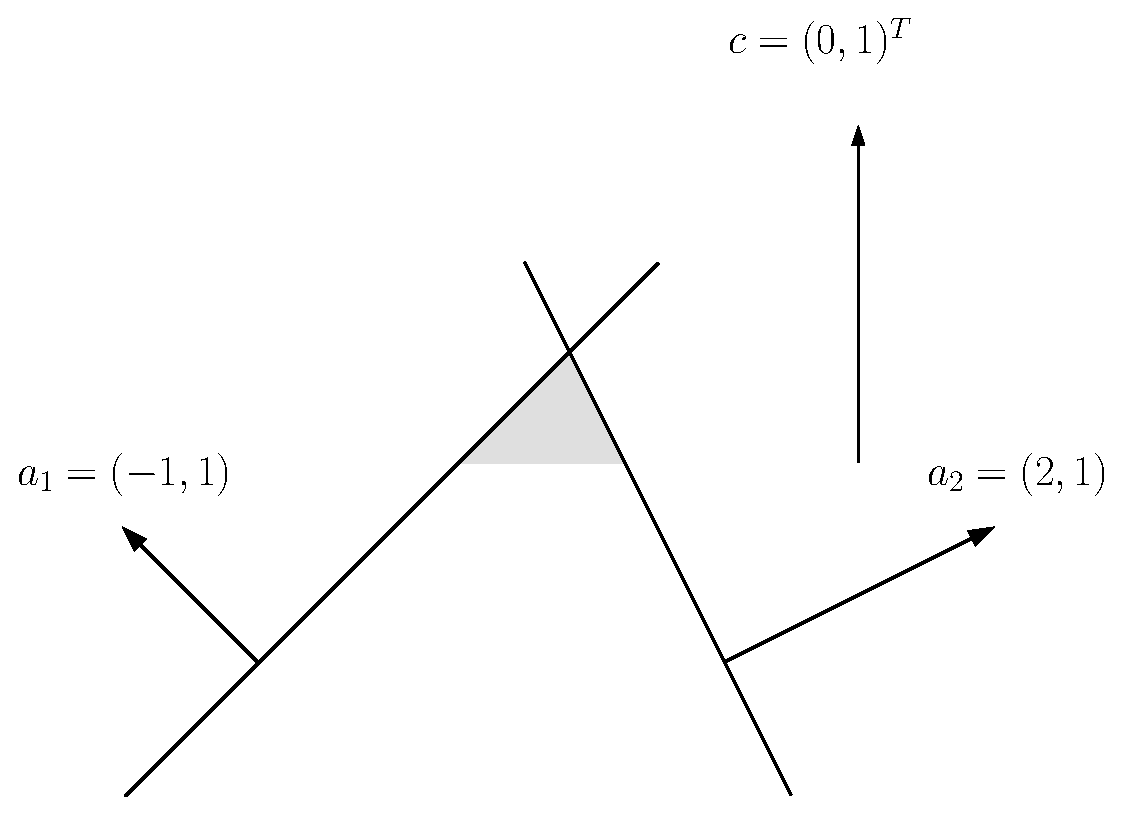
\includegraphics[height=5cm]{figures/example.eps}
      \caption{The initial roof  of Example~\ref{ex:1}.}
        \label{fig:ex:1.1}
    \end{center}    
  \end{figure}


\begin{example}
  \label{ex:1}
    
  Consider the linear program $\max\{x_2 \colon x \in \setR^n, \, (-1,1) x \leq
  1,\,  (2,1)x\leq1,\, (1,2) x \leq1 \}$. We start with the roof $B =
  \{1,2\}$ that consists of the first two inequalities see 
  Figure~\ref{fig:ex:1.1}. 
  
  \noindent 
  We compute first the  vertex $x^*_B$  which is the solution to the
  system 
  \begin{equation}
    \label{eq:19}
    \mat{-1 & 1 \\ 2 & 1}  x  = \mat{1\\1}.
  \end{equation}
  Thus the  vertex is the vector $x_B^* = \mat{0\\1}$.  
  
  \noindent 
  Next  we find that the halfspace $(1,2) x \leq1$ is not satisfied
  by $x_B^* = \mat{0\\1}$. We want to bring this index   into the new
  roof $B'$.
  
  \noindent 
  Step~3:
  Now we compute the solution  to the system 
  \begin{equation}
    \label{eq:20}
    \mat{-1 & 2 \\ 1 & 1} z = \mat{0\\1}
  \end{equation}
  and  find 
  $$z^* = \mat{2/3 \\ 1/3}.$$  
  
  Next we find a solution  to the system  
   \begin{equation}
     \label{eq:21}
    \mat{-1 & 2 \\ 1 & 1} y  = - \mat{1\\2}
  \end{equation} 
  and find  
  $$y^* = \mat{-1\\ - 1 }. $$
  
  \noindent
  The index set $J = \{1,2\}$ is not empty. The minimum~\eqref{eq:9} is
  achieved at  $j =2$. So the halfspace 
  $(2,1)x\leq1$ will leave the roof and $B' = \{1,3\}$. 
  This is also what we immediately see by
  looking at Figure~\ref{fig:ex:1.2}. 
   
\end{example}

  \begin{figure}[htbp]
    \begin{center}
      
      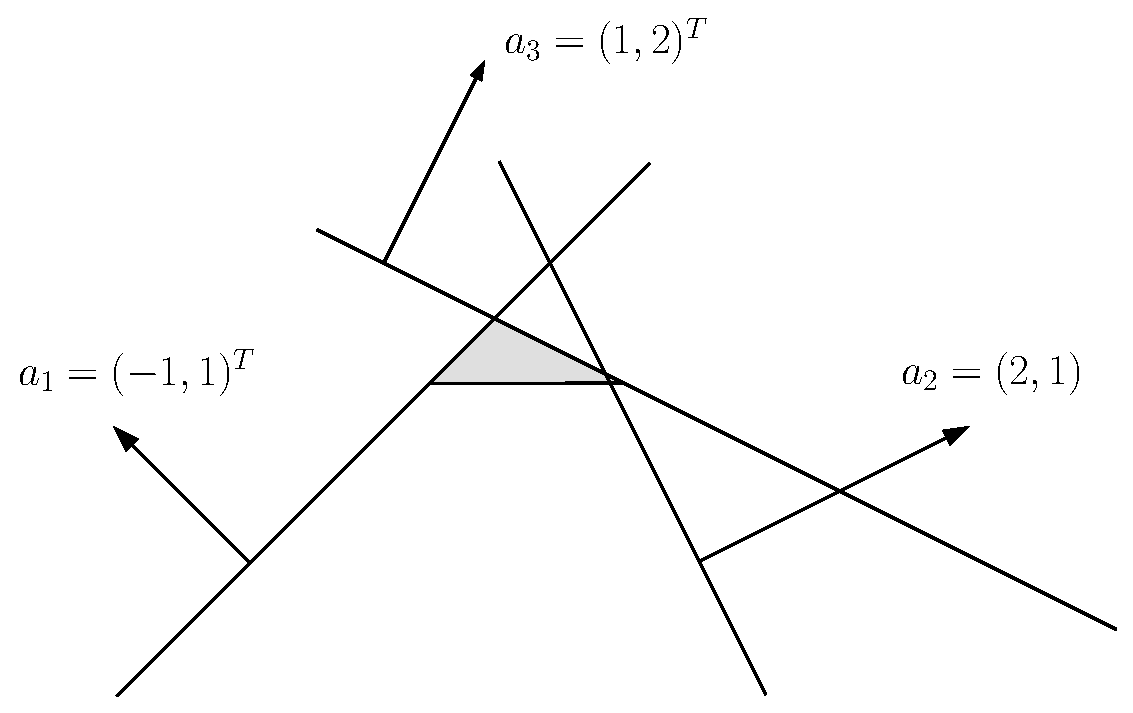
\includegraphics[height=5cm]{figures/example2.eps} 
      \caption{The new roof from  Example~\ref{ex:1}.} 
      \label{fig:ex:1.2}
    \end{center}
  \end{figure}


\noindent 

{ If $J = \emptyset$, } we assert that the linear program is infeasible based on
the following result. 

\begin{proposition}
  \label{thr:3}
  The half-spaces   $a_k\,x\leq b(k), \,k \in B $ and $a_i\,x\leq b(i)$
  define together an infeasible system 
  if and only   if $J = \emptyset$.
\end{proposition}

\begin{proof}
  
  If $J \neq \emptyset$, then   Lemma~\ref{lem:1} implies that the half-spaces
  $a_k\,x\leq b(k), \,k \in B $ and  $a_i\,x\leq b(i)$ define a feasible system. 

  
  The index set  $J$ is empty if and only if $y^*\geq0$.   
  We now show that, if $y^* \geq 0$, then the half-spaces $a_k\,x\leq b(k), \,k \in B $ and
  $a_i\,x\leq b(i)$ define an infeasible system. 
  Since  $\sum_{k \in B} y^*_k a_k + a_i = 0$  this assertion follows,
  once we have shown that  $\sum_{k \in B} y_k b(k) + b(i) < 0$. But 
  \begin{eqnarray*}
    \sum_{k \in B} y_k b(k) + b(i)  & = & \sum_{k \in B} y^*_k a_k\, x^*_B + b(i)  \\
               & <  & \sum_{k \in B} y^*_k a_k\, x^*_B + a_i\, x^*_B  \\ 
               & = &  \left(\sum_{k \in B} y^*_k a_k + a_i \right)\, x^*_B  \\ 
               & = &  0^T   x_B^* \\
               & = & 0. 
  \end{eqnarray*}
\end{proof}







% This algorithm which we have just described is called
% \emph{pivoting}. 
% Now we can describe the famous simplex algorithm which finds the
% lowest v-shape of a HPP. It simply keeps pivoting until one can
% assert  that  $\eh$ is infeasible or unbounded or until a lowest
% v-shape is found. 

% \begin{algorithm}[Simplex]~\\
%   \begin{tabular}{ll}
%     {\bf Input:}  & non-degenerate $\hpp(\eh,c)$ and a v-shape $\ev$\\
%     {\bf Output:} & lowest v-shape $\ev'$ \\
%     & or assertion that $\eh$ is infeasible 
%   \end{tabular}
  
%   \begin{enumerate}
%   \item $\wt{\ev} \gets \ev$
%   \item {\bf REPEAT}
%     \begin{enumerate}
%     \item Run {\bf Pivot} on $\wt{\ev}$
%     \item If this reveals that $\wt{\ev}$ is lowest v-shape
%       \begin{enumerate}
%       \item {\bf RETURN} $\wt{\ev}$
%       \end{enumerate}
%     \item If this reveals that $\eh$ is infeasible
%       \begin{enumerate}
%       \item {\bf RETURN} $\eh$ is infeasible
%       \end{enumerate}
%     \item If this returns v-shape $\ev'$ \label{xitem:2}
%       \begin{enumerate}
%       \item  $\wt{\ev} \gets \ev'$
%       \end{enumerate}
%     \end{enumerate}
%     \item {\bf UNTIL} 0
%   \end{enumerate}
% \end{algorithm}


% \begin{theorem}
%   \label{thr:4}
%   The simplex algorithm terminates after a finite number of steps on a
%   non-degenerate HPP. 
% \end{theorem}

% \begin{proof}
%   The only interesting step is~\ref{xitem:2}). The vertex of the new
%   v-shape is feasible for the old v-shape by
%   Proposition~\ref{prop:3}. Since the HPP is non-degenerate, this new
%   vertex has a strictly smaller objective function. Since there are
%   only a finite number of v-shapes, the simplex algorithm terminates. 
% \end{proof}

% This gives us also a proof of our strong duality theorem for
% non-degenerate HPP's. 






 \subsection{The degenerate case}
 \label{sec:degenerate-case}

 The termination argument for the non-degenerate case was that the
 value of the new roof  is strictly dropping and thus, that a
 roof can never be revisited. Since there are only a finite number
 of roofs, this implies that the simplex algorithm terminates.

 In the degenerate case, roofs could be revisited. This phenomenon
 is called \emph{cycling} and you are asked to construct such an
 example in the exercises. What can we do about it? The idea is  to change the
 objective vector $c \in \setR^n$ a little bit and turn it into a vector
 $c_\epsilon$ such that the following conditions hold. 

 \begin{enumerate}[1)]
 \item The linear program  
   \begin{equation}
     \label{eq:6}
      \max\{c_\varepsilon^Tx \colon  x \in  \setR^n, \, Ax \leq b\}
   \end{equation}
   has a roof.\label{xitem:19}
 \item Each non-roof of the linear program~\eqref{eq:28}  is a non-roof  of the
   linear program~\eqref{eq:6}. \label{xitem:18}  
 \item No roof of \eqref{eq:6} is degenerate. \label{xitem:20}
 \end{enumerate}


 Suppose we start with  an initial roof 
 $R$ at the beginning of the
 simplex algorithm and let ${A_R}\in \setR^{n\times n}$ be the matrix whose
 rows  are the vectors $a_i, \, i \in R$. 
 Notice that we implicitly assume that the set $R$ is ordered. We
 adhere to the following notation. For $i \in R$, the function $f_R(i)$
 denotes the position of $i$ in the ordered set $R$. For example, if
 $R = \{5,2,9\}$, then $f_R(5)=1$ and $f_R(9)=3$. 

 The system ${A_R}^T \,y =c$
 has a solution ${y^*}\geq0$, where some components of ${y^*}$ are zero
 if and only if $R$ is degenerate. 
  This is undesirable and we wish that ${y^*}$ is replaced by
 \begin{equation}
   \label{eq:7}
   {y^*} +  \mat{\epsilon \\ \epsilon^2 \\ \vdots \\\epsilon^n}
 \end{equation}
 for some $\epsilon>0$. Later it will
 become clear why we add the vector $(\epsilon,\ldots,\epsilon^n)^T$ instead of the vector
 $(\epsilon,\ldots,\epsilon)^T$. Now the vector~\eqref{eq:7} becomes a solution if we
 perturb $c$ and consider the vector 
 \begin{equation}
   \label{eq:18}
   c_\epsilon = c + {A_R}^T \mat{\epsilon \\ \epsilon^2 \\ \vdots \\\epsilon^n}
 \end{equation}
 instead, see figure~\ref{fig:perturb}. 
 \begin{figure}[h]
     \begin{center}{


    \psset{unit=.8cm}
    \begin{pspicture}(-1,-2)(5,4)
%      \showgrid
      \pspolygon[fillcolor=vlg,linecolor=vlg,fillstyle=solid](-1,4)(2,1)(2,-2)
      \rput(0,1){Roof $R$}
      \psline(2,-2)(2,1)
      \psline(-1,4)(2,1)
      \psline[linecolor=red,linewidth=1.5pt]{->}(2.5,1.5)(4.5,1.5)
      \rput(4.3,1.2){\red{$c$}}

      {
      \psline[linecolor=magenta,linewidth=1.5pt]{->}(2.5,1.5)(4.4,1.9)
      \rput(4.3,2.1){\magenta{$c_\varepsilon$}}
      }

      \psline[linecolor=blue]{->}(0,3)(1,4)
      \psline[linecolor=blue]{->}(2,-1)(3,-1)
%      \showgrid
    \end{pspicture}
\hfill 
    \begin{pspicture}(0,0)(4,4)
 %           \showgrid
%      \rput(-.2,-.2){$0$}
      \pspolygon[fillcolor=vlg,linecolor=vlg,fillstyle=solid](0,0)(4,0)(4,4)
      
      \rput(3,1.3){$\cone(A_R^T)$}
      
       \psline[linecolor=red]{->}(0,0)(2,0)
       
       {
          \psline[linecolor=magenta]{->}(0,0)(2.4,0.3)
       }
      \psline[linecolor=blue]{->}(0,0)(1,0)
      \psline[linecolor=blue]{->}(0,0)(1,1)
%      \showgrid
    \end{pspicture}
    }
    
  \end{center}

   \caption{An example of perturbation.}
   \label{fig:perturb}
 \end{figure}
If $\epsilon>0$, then $R$ is a non-degenerate roof  of
 the linear program~\eqref{eq:6}. Thus condition~\ref{xitem:19}) holds
 for any $\epsilon>0$. In 
 the sequel, we make $\epsilon$ smaller and smaller, such that also the
 conditions~\ref{xitem:18}) and~\ref{xitem:20}) will be satisfied. 



 Let us  first deal with condition~\ref{xitem:18}). Let 
 $B$ be a set of linear indices such that the vectors $a_i, \, i \in
 B$ are a basis of $\setR^n$ and suppose that $B$ is not a roof. We have
 to guarantee that $B$ is not a roof of the perturbed linear program. 

 Let $A_{B} \in  \setR^{n\times n}$ be the sub-matrix of $A$ that is defined
 by the rows of $A$ indexed by $B$. 
 Since $B$ is not a roof, the vector ${A_{B}}^{-T}\,c $ has a strictly
 negative component. Suppose that this component is the $i$-th
 component $(A_{B}^{-T}\,c)(i)<0$.  By choosing $\epsilon>0$ sufficiently small,
 we guarantee that   
 \begin{equation}
   (A_{B}^{-T}\,c_\epsilon)(i)  =  \left(A_{B}^{-T}\, c + A_{B}^{-T}A_R^T     \mat{\epsilon \\ \epsilon^2 \\ \vdots \\\epsilon^n}\right)(i)\label{eq:23}    <  0.               
 \end{equation}
               Thus condition~\ref{xitem:18}) is satisfied by choosing $\epsilon>0$
 sufficiently small. 

 For  condition~\ref{xitem:20}) we have to work only a little harder, and
 in fact, this is why we add the vector $(\epsilon,\ldots,\epsilon^n)$ instead of
 $(\epsilon,\ldots,\epsilon)$. Let $B$ be a roof  of \eqref{eq:6} 
 and let $A_{B} \in \setR^{n\times n}$ be again the above described
 sub-matrix. 
 We now argue that, if  $\epsilon$ is sufficiently small, then $A_{B}^{-T}c_\epsilon$
 does not have any component equal to  zero.  We are done then in
 showing that, for $\epsilon$ sufficiently small, the linear program~\eqref{eq:6} is
 non-degenerate. Because any  roof of~\eqref{eq:6}  will then be
 non-degenerate. 

 So let us inspect the vector 
 \begin{equation}
   \label{eq:24}
   A_{B}^{-T} c_\epsilon = A_{B}^{-T}c + A_{B}^{-T}\cdot {A_R}^T \mat{\epsilon \\ \vdots \\ \epsilon^n}. 
 \end{equation}
 Each component of \eqref{eq:24} is a nonzero polynomial with
 variable~$\epsilon$.  Nonzero, because $A_{B}$ and ${A_R}$ are non-singular
 matrices. It is well known, that a nonzero polynomial of degree~$n$
 has at most $n$ roots. Thus, for $\epsilon>0$, sufficiently  small, no
 component of~\eqref{eq:24} will be zero. 



 So the conditions~\ref{xitem:19}), \ref{xitem:18}) and
 \ref{xitem:20}) hold for $\epsilon>0$ sufficiently small. Thus we can
 modify a degenerate linear program into an equivalent non-degenerate
 linear program and apply the simplex algorithm to it.


 \begin{theorem}
   \label{thr:2}
   Let 
   \begin{equation}
     \label{eq:11}
        \max\{c^Tx \colon x \in \setR^n, \, Ax\leq b\}
   \end{equation}
   be a linear program. The simplex method
   terminates on the perturbed linear program~\eqref{eq:6}. It either
   returns  a roof
   $B$ of~\eqref{eq:11} and \eqref{eq:6} whose vertex $x^*_{B}$ is
   an optimal solution of~\eqref{eq:11} or it asserts
   that~\eqref{eq:11} is infeasible. 
 \end{theorem}
 

 \begin{proof}
   The simplex method terminates on~\eqref{eq:6} since this linear
   program is non-degenerate. If it asserts that~\eqref{eq:18} is
   infeasible, then it also follows that \eqref{eq:11} is infeasible,
   since the perturbation only changes the objective-function vector.
   
   If it returns a roof $B$ of \eqref{eq:6}, then this is also a roof
   of~\eqref{eq:11} by condition~\ref{xitem:18}). Furthermore, the
   vertex $x^*_{B}$ is feasible for~\eqref{eq:11}. It follows from
   weak  duality   (Theorem~\ref{thr:6}) that $x^*_{B}$ is an optimal
   solution of~\eqref{eq:11}.  \qed 
 \end{proof}





   \subsection{The lexicographic pivot rule}
   \label{sec:lexic-pivot-rule}


   We now show that we do not have to physically perform the
   perturbation which sends $c$ to $c_\epsilon$, but instead describe a rule to
   choose the leaving index from the possible candidates for which the
   minimum in~\eqref{eq:9} is attained. Rules for entering and exiting
   indices are called \emph{pivoting rules}.  Recallthat for  $i \in
   B$, the function $f_B(i)$ 
   denotes the position of $i$ in the ordered set $B$. For example, if
   $B = \{5,2,9\}$, then $f_B(5)=1$ and $f_B(9)=3$. We need to define
   the lexicographic order. A vector $u \in \setR^n$ is lexicographically
   smaller than a vector $v \in \setR^n$ if $u\neq v$ and the first nonzero
   component of $v-u$ is positive.  We write $u<_{lex}v$ and if
   $u<_{lex}v$ of $u=v$ we write $u\leq_{lex}v$. 
   
   

   \begin{algorithm}{Simplex algorithm with lexicographic pivoting
       rule} \label{alg:3}
     
     \begin{tabbing}
       {\bf Input:} $A \in \setR^{m\times n}$, $c \in \setR^n$, $b
       \in \setR^m$
       $R\subseteq\{1,\ldots,n\}$  initial roof \\
      {\bf Output:}  $B$ optimal roof  or assert that LP is infeasible\\
      \\ 
      $B := R$  \\
       {\bf while } \= $\exists i \in\{1,\ldots,n\}$ with $a_ix^*_B >b_i$ \\
                   \> compute solution  \=  $y^*$ of \\
\> \>    $\Sigma_{k \in  B}  a_k y_k   =  -a_i $ \\
\> Compute  $J  = \{ k \in B \colon y^*_k <0\}$ \\

\> {\bf if }   $J = \emptyset$ assert {\bf LP not feasible} \\
\> {\bf else}\=      \\
\> \> Choose \emph{unique}  $j  \in J$ for which the vector \\
\> \> $\frac{(A_B^{-T} [c \mid {A_R}^T])_{f_B(j)}}{  - y^*_j}$ is \emph{ lexicographically
  minimal} \\
\> \> $B := B \textbackslash{} \{j\} \cup\{i\}$       
    \end{tabbing}
  \end{algorithm}
  % 
\marginpar{Change $T$ to $R$}
  A close inspection reveals that this algorithm only mimics the simplex
  algorithm on the perturbed problem~\eqref{eq:6} if $\varepsilon$ is
  arbitrarily close to $0$. This is because the first component of the
  vector $(A_B^{-T} [c \mid {A_R}^T])_{f_B(j)}$ is $z^*_j$, where $z^*$ is
  the solution of \eqref{eq:5} and if one replaces $c$ in
  \eqref{eq:5} with $c_\varepsilon$, the corresponding $z^*_j$ is simply 
  \begin{equation}
    \label{eq:50}
    (A_B^{-T} [c \mid {A_R}^T])_{f_B(j)} \mat{1\\\varepsilon\\\varepsilon^2 \\ \vdots\\\varepsilon^n}. 
  \end{equation}
  
%    So let us inspect step~3 for the perturbed problem
%    $\hpp(\eh,c_\epsilon)$. The solution $v^*$ to~(\ref{eq:17}) is the same for
%    the perturbed and non-perturbed problem. However, the solution
%    to~(\ref{eq:5})  is equal to 
%    \begin{equation}
%      \label{eq:25}
%      y^* + A^{-T} \cdot \wt{A} \mat{\epsilon \\ \vdots \\ \epsilon^n},
%    \end{equation}
%    where we neglect the last zero component. 
%    Now again, let $I \subseteq\{1,\ldots,n\}$ be the in $v^*(i)<0$. In the perturbed
%    problem, we determine the index $\ell \in I$ such that 
%    \begin{equation}
%      \label{eq:26}
%      - (y^*(\ell) + A^{-T} \cdot \wt{A} \mat{\epsilon \\ \vdots \\ \epsilon^n})(\ell) / v^*(\ell) 
%    \end{equation}
%    is minimal. In the unperturbed problem, there could be a set $L\subseteq I$ of
%    indices, for which the minimum is attained. 

%    \begin{definition}[Lexicographic order, $\geq_{\lex}$]
%      \label{def:2}
%      Let $u$ and $v$ be vectors of $\setR^n$. We say that $u\geq_{\lex}v$ if the
%      first nonzero entry of $u-v$ is positive. We say that $u$ is
%      \emph{lexicographically larger} than $v$. If $u \neq v$ then we write $u>_{\lex}v$. 
%    \end{definition}
%    %
%    In the following we write $r_j(\epsilon)$ for the $j$-th polynomial  
%    \begin{equation}
%      \label{eq:27}
%      -(y^*(j) + A^{-T} \cdot \wt{A} \mat{\epsilon \\ \vdots \\ \epsilon^n})(j) / v^*(j), \, j \in L.
%    \end{equation}
%    %
%    This polynomial is defined by its coefficient vector $r_j\in
%    \setR^{n+1}$.  The vector $r_j$ is the $j$-th row of the matrix 
%    $- \left( y^*, A^{-T} \cdot \wt{A}\right)$ divided by $v^*(j)$. 
%    We imitate the perturbed choice by choosing the index $\ell$ such that 
%    $r_j$ is lexicographically smallest. 
%    Let us spend a little more time in explaining why.  Let $r_\ell$
%    be this lexicographically smallest vector. Since $ A^{-T} \cdot \wt{A}$ is
%    non-singular, each row $r_j$ is strictly larger than $r_\ell$. 
%    This means that $r_j - r_\ell$ is a vector whose first nonzero component
%    is strictly positive. Thus $(r_j - r_\ell)(\epsilon) >0$ for $\epsilon$ sufficiently
%    small. 


%    Thus the following lexicographic  pivoting rule guarantees the
%    termination of the simplex method. 

%    \begin{xitemize}
%    \item   Determine the set $L\subseteq I$ for which the minimum 
%      \begin{displaymath}
%        \min_{i \in I} -  y^*(i)/v^*(i)
%      \end{displaymath}
%      is attained.  
%      \item Choose the index $\ell \in L$  such that 
%      \begin{displaymath}
%        \frac{\ell\mbox{-th row} - \left( y^*, A^{-T}\cdot\wt{A}\right)}{v^*(\ell)} \leq_\lex 
%        \frac{j\mbox{-th row} - \left( y^*, A^{-T} \cdot \wt{A}\right)}{v^*(j)} \mbox{ for each } j \in L.
%      \end{displaymath}
%      \item The $\ell$-th halfspace leaves the v-shape. 
%    \end{xitemize}



  \section{Phase~I, finding an initial roof}
  \label{sec:phase-i-finding}


  So far, we always started with an initial roof. Where do we get 
  it  from?  This is where Phase~I of the simplex method is put to
  work. Above, we described Phase~II.   First we prove a little lemma. 
  
  \begin{lemma}
    \label{lem:3}
    If the linear program~\eqref{eq:28} is feasible and bounded, then
    it has an optimal roof. In particular, a feasible and bounded
    linear program has an optimal solution.
  \end{lemma}
  
  \begin{proof}
    We change the linear program~\eqref{eq:28} by adding the
    additional constraint $c^Tx \leq M+1$, where $c^Tx\leq M$ is valid for
    all feasible solutions. We then have a (degenerate) roof by
    choosing this inequality together with any subset of   $n-1$
    constraints whose normal-vectors together with $c$ form a basis of
    $\setR^n$. The     simplex algorithm will find an optimal roof. \qed 
  \end{proof}


  We now form an auxiliary linear program. Observe that the linear
  program 
  \begin{equation}
    \label{eq:22}
    \max\{c^Tx \colon x \in \setR^n, \, Ax\leq b\}
  \end{equation}
  has a roof if and only  
  if the linear program $\max\{c^Tx \colon x \in \setR^n, \,Ax\leq0\}$ has a
  roof.  The latter linear program is feasible since $0$ is a feasible
  solution. Furthermore, $0$ is an optimal solution of this linear
  program if and only if it has a roof. This is what we check with the
  simplex algorithm on the auxiliary program 
  \begin{equation}
    \label{eq:14}
    \max\{c^T x \colon x \in \setR^n, \, Ax\leq0, \, c^Tx \leq 1\}
  \end{equation}
  and we start with a (possibly) degenerate roof involving the
  inequality $c^Tx\leq1$ and $n-1$ of the constraints of $Ax\leq0$ whose
  normal-vectors, together with $c$ form a basis of $\setR^n$. The
  simplex algorithm terminates with an optimal roof. If the roof has
  vertex $0$, then we have found a roof of the original linear
  program~\eqref{eq:22} and can start the simplex algorithm for it. If
  the roof of Phase~I still contains the inequality $c^Tx\leq1$, then
  the original linear program~\eqref{eq:22} does not have any
  roof. This either means that the program is infeasible or
  unbounded. 
  
%   We now form an auxiliary linear program. Let $C^+$ and $C^-$ be the sets of indices
%   $C^+ = \{i\in\{1,\ldots,n\}\colon c(i) \geq0 \}$
%   $C^-=\{i\in\{1,\ldots,n\}\colon c(i)<0\}$.  The auxiliary linear program is 
%   \begin{equation}
%     \label{eq:12}
%     \max\{c^Tx \colon x \in \setR^n,\,  Ax\leq0, x(i) \leq1, \, i \in C^+, \, -x(i) \leq1, \, i \in C^-\}. 
%   \end{equation}

%   Notice that this linear program  is feasible and has a roof, namely
%   the inequalities
%   \begin{equation}
%     \label{eq:13}
%        x(i) \leq1, \, i \in C^+, \, -x(i) \leq1, \, i \in C^-.
%   \end{equation}
% %
%   The vertex $x^*$ of each roof that 
%   contains one of the inequalities~\eqref{eq:13} has a positive
%   objective value $c^Tx^*$. On the other hand, a roof  of
%   \eqref{eq:28}  yields a roof of~\eqref{eq:12}  with vertex $x^*=0$.
%   We start the simplex algorithm on this auxiliary linear program. If
%   we obtain a 
%   roof $B$ with vertex $x^*$ such that $c^Tx^*>0$, then the original
%   linear program  does not have roofs. Otherwise, we have identified
%   a subset  $B' \subseteq B$ of linear independent halfspaces  such that $c$ is a
%   conic combination of the normal-vectors of these half-spaces. If
%   $|B'|<n$,  we complete 
%   $B'$ to a degenerate roof $\wt{B}$ of the original linear program
%   and start the simplex algorithm on $\wt{B}$. 


%   \section{The running time of the simplex method}
%   \label{sec:running-time-simplex}


%   Starting at a v-shape $\ev$, it may happen, that one basically visits
%   all v-shapes of $\hpp(\eh,c)$ before one arrives at the lowest
%   v-shape. The number of v-shapes is bounded by $\binom{m}{n} =
%   \bigO(m^n)$. This is {\bf exponential} in the dimension. Thus the
%   simplex algorithm runs in polynomial time if the dimension is
%   fixed. We will see later, that there exists an algorithm, which solves
%   the highest point problem in polynomial time, even if the dimension
%   varies. 

%   However, the simplex method performs very well in practice. 

%   We close this section with a larger example.
%   \begin{example}
%     We consider a larger example with several iterations of the simplex
%     algorithm. Our goal is to solve a linear program~\eqref{eq:28} with 
%     \begin{displaymath}
%       A = \begin{pmatrix} 2& 4& 3 \\ 3& 1& 4 \\ 1& 2& 2 \\ 1& 0& 0 \\ 0&
%           1& 0 \\ 0& 0& 1 \end{pmatrix},\,    
%         b = \begin{pmatrix}-5\\ -3\\ -2 \\0 \\0 \\0 \end{pmatrix}\, ,
%         c = \begin{pmatrix} 5 \\ 9 \\ 10          \end{pmatrix}. 
%     \end{displaymath}
%   %
%     The set of row-indices is $\{1,2,3,4,5,6\}$. We start with the roof
%     $\{4,5,6\}$. 
%     \begin{xitemize}
%     \item[$\{4,5,6\}$]  
%     \end{xitemize}

  


  
%   \end{example}



\section{The full column-rank assumption}
\label{sec:full-column-rank}

There is one thing that we still have to deal with. The simplex
algorithm is based on the assumption that the columns of $A$ are
linearly independent. %  We use the following lemma from linear algebra
% to make this assumption without loss of generality. 
We now argue that this assumption can be made without loss of
generality. 

Suppose that $A$ can be written as $[A_1 \mid A_2]$ with $A_1 \in \setR^{m\times k}$
and $A_2 \in \setR^{m\times(n-k)}$ where the columns of $A_1$ are linearly
independent and each column of $A_2$ is a  linear combinations of the
columns of $A_1$.  We also write $c = \smat{c_1\\c_2}$ with $c_1 \in
\setR^k$ and $c_2 \in \setR^{n-k}$ and consider the linear program 
\begin{equation}
  \label{eq:32}
  \max\{c_1^Tx_1 \colon x_1 \in \setR^{k} , \, A_1x_1\leq b\}
\end{equation}


Since each column of $A_2$ is a linear combination of the columns of
$A_1$, there exists a uniquely determined  matrix $U \in \setR^{k\times(n-k)}$
with $A_2 = A_1\cdot U$.  


\begin{lemma}
  \label{lem:7}
  The linear program~\eqref{eq:32} is feasible if and only if the
  linear program~\eqref{eq:28} is feasible. 
\end{lemma}


\begin{proof}
  Suppose  that $x^* =\smat{x_1^*\\x_2^*}$ is a feasible
  solution of \eqref{eq:28}, i.e.,  $A_1x_1^* + A_2 x_2^*\leq b$. But
  $A_1x_1^* + A_2x_2^* = A_1 (x_1^* + U \cdot x_2^*)$ which yields a
  feasible solution of~\eqref{eq:32}. Likewise we see that any
  solution $x_1^*$ of $A_1x_1\leq b_1$ can be extended to a feasible
  solution $\smat{x^*_1 \\ 0}$ of~\eqref{eq:28}. \qed 
\end{proof}


\begin{lemma}
  \label{lem:8}
  If~\eqref{eq:32} is feasible and if $c_2^T \neq c_1^T\cdot U$, then
  \eqref{eq:28} is unbounded. 
\end{lemma}


\begin{proof}
  Since~\eqref{eq:32} is feasible, then also~\eqref{eq:28} is
  feasible. Let $x^*$ thus be a feasible solution
  of~\eqref{eq:28}. Then $x^* + \mu \smat{-U v \\ v}$ is feasible for
  any $v \in \setR^{n-k}$ and $\mu \in \setR$. Let $v$ satisfy $c_2^Tv \neq 0$,
  then $c_1^T (-U) v + c_2^T v \neq 0$ which implies that \eqref{eq:28}
  is unbounded. \qed 
\end{proof}


The idea is thus to re-order the columns of $A$ such that the first
$k$ columns are linearly independent and the last $n-k$ columns are
linear combinations of the first $k$ columns. This also yields a
matrix $U$ and we now solve the linear program~\eqref{eq:32} with the
simplex algorithm. If it is infeasible or unbounded, then so is the
linear program~\eqref{eq:28}. Otherwise the simplex algorithm finds an
optimal solution $x_1^*$  of~\eqref{eq:32}. If $c_2^T = c_1^T \cdot U$
then this optimal solution $\smat{x_1^*\\0}$ is also an optimal
solution of the linear program~\eqref{eq:32}. This is because a
feasible solution $\smat{x_1^*\\x_2^*}$ of \eqref{eq:28} yields a
feasible solution $x_1^*+U\cdot x_2^*$ of \eqref{eq:32} with same objective
value $c_1^T(x_1^* + U x_2^*) = c_1^Tx_1^* + c_2^Tx_2^*$. 

% \begin{lemma}
%   \label{lem:6}
%   Let $A \in \setR^{m\times n}$ where the first $k\leq n$ columns are linearly
%   independent and the last $n-k$ columns of $A$ are obtained as linear
%   . There exists an invertible
%   matrix $U \in \setR^{n\times n}$ with $A\cdot U = [B | 0]$, where $B$ has full
%   column-rank.
% \end{lemma}
% Here $0$ stands for the all zero matrix with $m$ rows and $n-k$
% columns. 
% This lemma is proved in a course on linear algebra. The algorithm with
% which one can compute the matrix $U$ is Gaussian elimination. We use
% this to compute from  the linear program
% \begin{equation}
%   \label{eq:30}
%   \max\{c^Tx \colon  x \in \setR^n, \,Ax \leq b\}
% \end{equation}
% the linear program
% \begin{equation}
%   \label{eq:31}
%   \max\{c_1^Ty \colon  y \in \setR^{n-k}, \, By \leq b\},
% \end{equation}
% where $c^T = (c_1^T,c_2^T)$ with $c_1 \in \setR^{n-k}$. 
% We observe that this linear program is feasible if and only
% if~\eqref{eq:30} is feasible. 


\section*{Exercises}

\begin{enumerate}[1)]
\item \label{xitem:8}
  Show that the linear program~\eqref{eq:29} that is defined by a roof
  is always feasible. 
\item  Let $B$ be a roof of the linear program~\eqref{eq:28} and 
  consider the system of linear equations
  \begin{displaymath}
    a_{j}^Tx = -1, a_i^Tx=0, \, i \in B\setminus\{j\}
  \end{displaymath}
  for an index $j \in B$. 
  Let $x^*$ be a feasible solution to the roof-linear
  program. Show that  $x^* + \lambda \cdot v$ is also feasible for each 
  $\lambda>0$.  \label{xitem:9} 


\item Prove Proposition~\ref{prop:2}. \label{xitem:11}


\item 
  \label{sec:high-point-probl}
  Let $B$ be a roof with vertex $x^*_B$. Show that the 
   set of  feasible points $\{x \in \setR^n \colon a_i^Tx\leq b(i), \, i\in B\}$
   of the roof is of the form 
  $x_B^* + \cone\{r_1,\ldots,r_n\}$ for some suitable vectors $r_i \in
  \setR^n$, $i=1,\ldots,n$. 

\item A cone $C\subseteq \setR^n$ is \emph{pointed} if it does not contain a line: There are no vectors $x\in C$, $v\in \setR^n$ such that $x+\lambda v\in C$ for all $\lambda\in \setR$.

Prove the following variant of Carath\'eodory's theorem. 
Given some set  $X\subseteq \setR^n$, $|X|>n$ such that $\operatorname{cone}(X)$ is pointed.
For any $x \in \operatorname{cone}(X)$, there exist at least two
  different subsets $X_1,X_2\subseteq X$ with  $|X_1| = |X_2| = n$ such that $x\in \operatorname{cone}(X_1)\cap \operatorname{cone}(X_2)$.
 \label{xitem:12}
\item 
Consider the problem
\begin{eqnarray}
\label{row0}    \max & z & \\
\label{row1}    \text{s.t.} &  x+2y      & \leq -3 \\
\label{row2}        &  -2x - 3y  & \leq 5 \\
\label{row3}        & -2x -y  +2z& \leq -1 \\
\label{row4}	    &  3x+y  & \leq 2 \\
\label{row5}	    &  x  & \leq 0 \\
\label{row6}	    &  y  & \leq 0 \\
\label{row7}	    &  z  & \leq 0.
\end{eqnarray}
Assume that we perform the simplex method, and at some point have the roof given by the rows \eqref{row1}, \eqref{row6} and \eqref{row7}.
Figure \ref{fig:IllustrDegeneracyExercise} shows the situation in the 2-dimensional subspace given by the hyperplane $z=0$.

Show that the simplex algorithm might not terminate, by giving a cycling sequence of roofs that might be selected by the simplex method.
Explain why your sequence is valid (it is sufficient to give drawings here, you do not need to compute the roof vertices explicitly).

\emph{Hint: Never let \eqref{row7} leave the roof. Then it is sufficient to consider the subspace as in the illustration.}

\begin{figure}[hbt]

  \begin{center}
\begin{pspicture}(-4cm,-4cm)(4cm,4cm)
\psset{unit=0.4cm}
\pspolygon[fillcolor=vlg,linecolor=vlg,fillstyle=solid](-10,3.4)(-10,2.9)(10,-7.1)(10,-6.6)
\pspolygon[fillcolor=vlg,linecolor=vlg,fillstyle=solid](-10,5.1)(-10,5.6)(10,-7.73)(10,-8.23)
\pspolygon[fillcolor=vlg,linecolor=vlg,fillstyle=solid](-4.4,10)(-3.9,10)(6.1,-10)(5.6,-10)
\pspolygon[fillcolor=vlg,linecolor=vlg,fillstyle=solid](-2.76,10)(-3.26,10)(3.5,-10)(3.9,-10)
\pspolygon[fillcolor=vlg,linecolor=vlg,fillstyle=solid](-0.1,10)(-0.6,10)(-0.6,-10)(-0.1,-10)
\pspolygon[fillcolor=vlg,linecolor=vlg,fillstyle=solid](-10,-0.1)(-10,-0.6)(10,-0.6)(10,-0.1)


      \psline(-10,3.5)(10,-6.5) %first
      \psline(-10,5)(10,-8.33) %second
      \psline(-4.5,10)(5.5,-10) % third
      \psline(-2.66,10)(4,-10) % fourth
      \psline(0,10)(0,-10) % fifth
      \psline(-10,0)(10,0) % sixt

\rput(-9.5,2.2){\eqref{row1}}
\rput(-9.5,6){\eqref{row2}}
\rput(-5.2,9.5){\eqref{row3}}
\rput(-1.86,9.5){\eqref{row4}}
\rput(0.6,9.5){\eqref{row5}}
\rput(-9.5,-1){\eqref{row6}}
      
      \psdot[linecolor=red](-3,0)
      %\psline[linecolor=blue]{->}(0,3)(1,4)
      %\psline[linecolor=blue]{->}(2,-1)(3,-1)
%      \showgrid
\end{pspicture}
\end{center}
\caption{The halfspaces defined by system \eqref{row0} in the subspace
  $\{(x,y,0)~:~x,y\in \setR\}$.}
\label{fig:IllustrDegeneracyExercise}
\end{figure}


\end{enumerate}




%%% Local Variables: 
%%% mode: latex
%%% TeX-master: "lecture"
%%% End: 
